% =============================================================================
% Section 4.7: Assessment and Quiz Module
% =============================================================================

\section{Assessment and Quiz Module}
\label{sec:assessment-module}

\subsection{Functional Description}

The Assessment module is one of the most domain-rich contexts in NexaLearn. It manages the full lifecycle of quizzes, questions, and learner attempts. The module supports multiple question types (multiple-choice, true-or-false, short-answer), configurable passing scores, time limits, randomisation, and both automatic and AI-assisted (short-answer) grading. Quiz results feed into the Progress module for learner analytics and into the Reviews module for peer assessment of short-answer responses.

\subsection{Quiz Authoring Aggregate}

The \texttt{QuizEntity} aggregate root enforces the invariants of quiz authoring:

\begin{lstlisting}[caption=QuizEntity Aggregate Root Showing Invariants,label=lst:quiz-entity]
export class QuizEntity {
  constructor(
    public readonly id: string,
    public lessonId: string,
    public title: string,
    public instructions: string,
    public passingScore: number,       // 0--100
    public maxAttempts: number,         // 0 = unlimited
    public timeLimitMinutes: number | null,
    public shuffleQuestions: boolean,
    public questions: QuestionEntity[],
    public status: QuizStatus,
  ) {}

  addQuestion(question: QuestionEntity): void {
    if (this.status !== QuizStatus.DRAFT)
      throw new BusinessRuleViolation('Cannot modify published quiz');
    this.questions.push(question);
  }

  publish(): void {
    if (this.questions.length < 1)
      throw new BusinessRuleViolation('Quiz must have at least 1 question');
    if (this.questions.some(q => q.options.length < 2))
      throw new BusinessRuleViolation('Each question needs at least 2 options');
    this.status = QuizStatus.PUBLISHED;
  }

  gradeAttempt(
    answers: AnswerDto[],
    shortAnswerGradingService: ShortAnswerGradingService,
  ): QuizAttemptEntity {
    let correctCount = 0;
    const gradedAnswers = answers.map((answer) => {
      const question = this.questions.find(q => q.id === answer.questionId);
      if (!question) throw new BusinessRuleViolation('Question not found');

      if (question.type === QuestionType.SHORT_ANSWER) {
        return {
          questionId: question.id,
          status: 'PENDING_GRADING',
          pointsAwarded: null,
        };
      }

      const isCorrect = question.correctOptionId === answer.selectedOptionId;
      if (isCorrect) correctCount++;
      return {
        questionId: question.id,
        selectedOptionId: answer.selectedOptionId,
        isCorrect,
        pointsAwarded: isCorrect ? question.points : 0,
      };
    });

    const score = Math.round((correctCount / this.questions.length) * 100);
    const passed = score >= this.passingScore;

    const hasPendingGrading = gradedAnswers.some(a => a.status === 'PENDING_GRADING');

    return QuizAttemptEntity.create({
      quizId: this.id,
      answers: gradedAnswers,
      score,
      passed,
      status: hasPendingGrading ? QuizAttemptStatus.IN_PROGRESS : QuizAttemptStatus.GRADED,
    });
  }
}
\end{lstlisting}

The aggregate root is the sole authority for grading: it receives learner answers, computes scores by comparing against the correct option for each multiple-choice question, and flags short-answer questions for asynchronous AI grading.

\subsection{Quiz Attempt Lifecycle}

Figure~\ref{fig:quiz-attempt-statemachine} shows the states of a quiz attempt.

\begin{figure}[H]
  \centering
  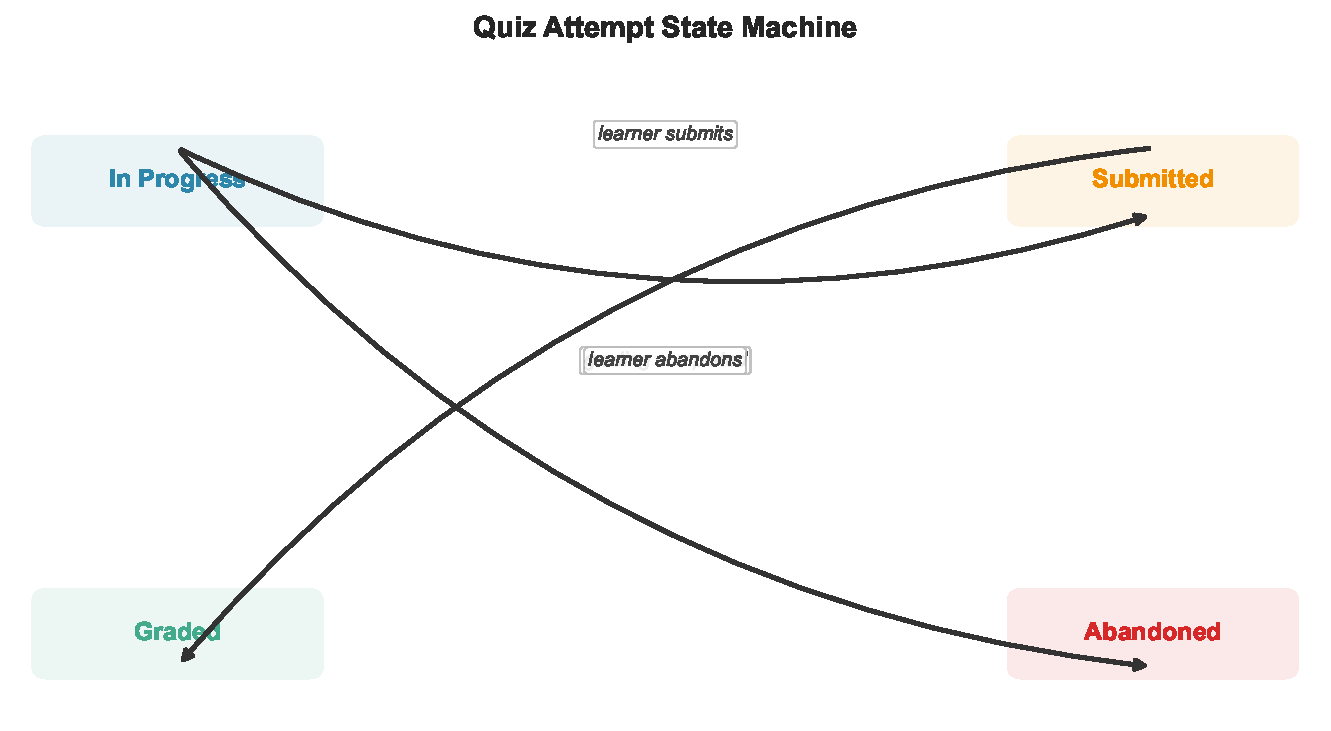
\includegraphics[width=0.7\textwidth]{images/statemachines/quiz_attempt_statemachine.pdf}
  \caption{Quiz Attempt State Machine}
  \label{fig:quiz-attempt-statemachine}
\end{figure}

When a learner starts a quiz, an attempt is created in IN\_PROGRESS state with a snapshot of the quiz questions (ensuring the quiz cannot change mid-attempt). When the learner submits, the attempt transitions to SUBMITTED. If all questions are auto-gradable (multiple-choice, true-or-false), the attempt is graded synchronously and transitions to GRADED. If the quiz includes short-answer questions, the attempt remains in SUBMITTED while the grading callback is awaited. When the AI pipeline responds, the attempt transitions to GRADED and the updated score is persisted. Learners may also abandon an attempt, transitioning it to ABANDONED.

\subsection{Asynchronous Short-Answer Grading}

Short-answer questions cannot be graded by simple string comparison---the learner's answer may be semantically correct regardless of exact wording. The Assessment module delegates grading to an LLM (configured per deployment as OpenAI GPT-4 or a self-hosted alternative). The grading prompt includes the question stem, the instructor-provided rubric, and the learner's answer, and returns a grade (0--100), a justification, and optionally feedback for the learner. The grader endpoint is call-back authenticated using the same HMAC pattern described in Section~\ref{sec:ai-pipeline-module}. Until grading completes, the learner sees a ``Grading in progress'' status. When grading finishes, the learner is notified, and the updated score propagates to the Progress module via an outbox event.
